\documentclass{beamer}

\usetheme{Antibes}
%\usetheme{split}
% this is a template for slides using beamer package
% adapted from slides written by Ramon Medrado
% first version: Ana Bazzan
\usecolortheme[RGB={120,0,0}]{structure}
\setbeamertemplate{blocks}[rounded][shadow=true]
\usepackage[utf8]{inputenc}   % pacote para acentuao
\usepackage{amsmath}
%% Listagens de código
\usepackage{listings}
\usepackage{color}
% \usepackage{caption}

\setbeamertemplate{footline}[frame number]
\setbeamertemplate{navigation symbols}{}
\setbeamertemplate{bibliography item}[text]

\definecolor{codegreen}{rgb}{0,0.6,0}
\definecolor{codegray}{rgb}{0.5,0.5,0.5}
\definecolor{codepurple}{rgb}{0.58,0,0.82}
\definecolor{backcolour}{rgb}{0.95,0.95,0.92}
 
\lstdefinestyle{mystyle}{
    % backgroundcolor=\color{backcolour},   
    commentstyle=\color{codegreen},
    keywordstyle=\color{magenta},
    numberstyle=\tiny\color{codegray},
    stringstyle=\color{codepurple},
    basicstyle=\scriptsize,
    breakatwhitespace=false,         
    breaklines=false,                 
    captionpos=b,                    
    keepspaces=true,                 
    numbers=left,                    
    numbersep=3pt,                  
    showspaces=false,                
    showstringspaces=false,
    showtabs=false,                  
    tabsize=2
}
\lstset{style=mystyle}

\setbeamerfont{caption}{size=\tiny}

\beamertemplateballitem

\begin{document}
\title
{Implementing a mobility scenario using SDN and Ryu Framework}


\author
{Iulisloi Zacarias \\ Janaína Schwarzrock}

\institute
{
  Instituto de Informática\\
  Universidade Federal do Rio Grande do Sul (UFRGS)
}

\date[CMP182]
{CMP182 – Redes de Computadores I, 2016/I \\
\scriptsize Prof. Dr. Edison Pignaton de Freitas \\
            Prof. Dr. Luciano Paschoal Gaspary}

% UFRGS Logo
\logo{
\includegraphics[scale=0.3]{images/inf}}


% If you wish to uncover everything in a step-wise fashion, uncomment
% the following command: 

%\beamerdefaultoverlayspecification{<+->}


% Slide de Título (Capa)
\frame[plain]{\titlepage}

% Slide de Resumo (Outline)
\frame{
	\frametitle{Outline}
	\tableofcontents
}

\section{Introduction}

\subsection{Scenario}

% ----------------------------------------------------------------
\begin{frame}{Scenario Characterization}
\begin{itemize}
  \item Proposed mobility scenario
  \item A stream video server
  \item Clients play the video streamed by the server
  \item Hosts can disconnect and connect from switches / access points 
\end{itemize}
\end{frame}

% ----------------------------------------------------------------
\begin{frame}{Scenario Diagram (Zone)}
	\begin{figure}
	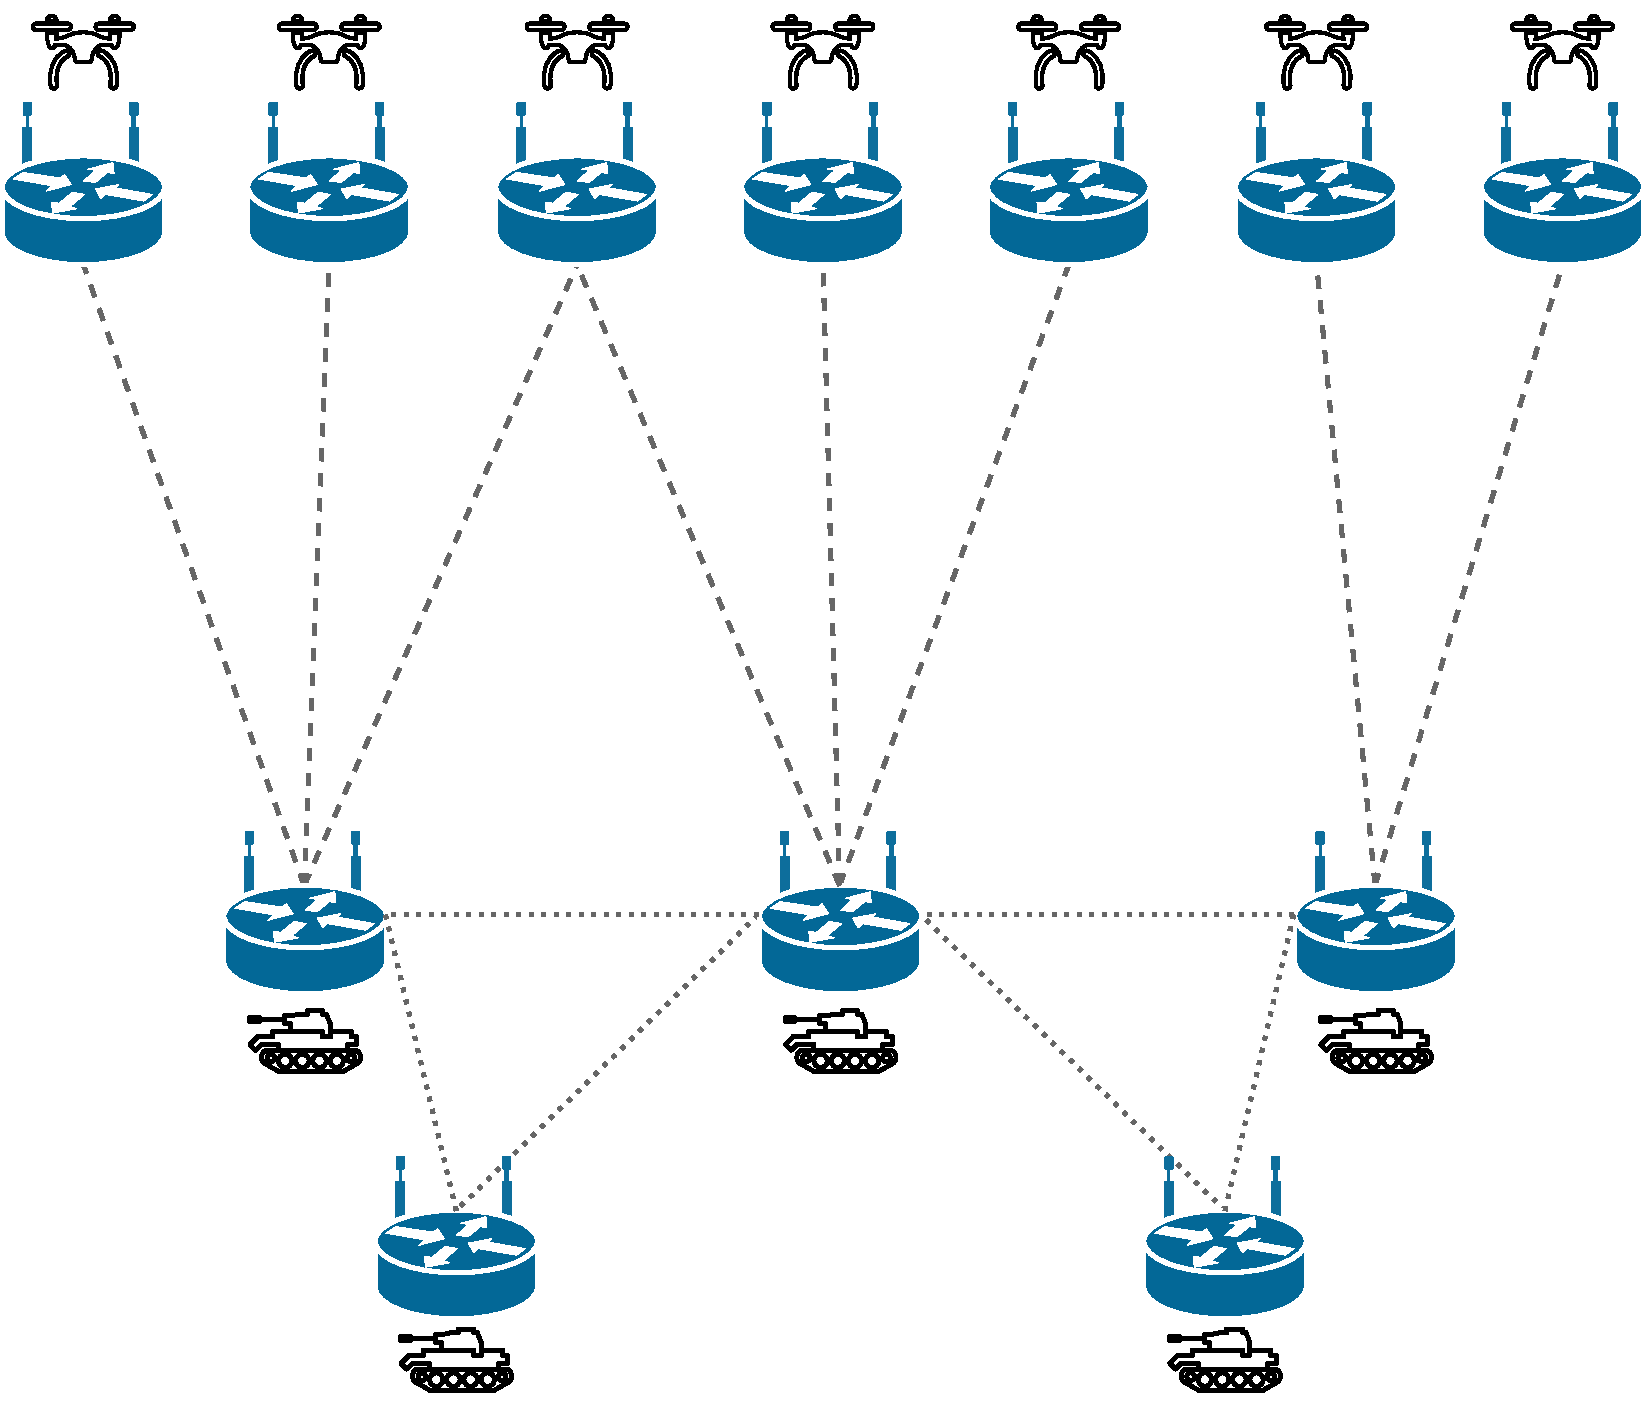
\includegraphics[scale=0.2]{images/forcas_armadas_2.pdf}
    \tiny
	\caption{Dashed and dotted lines represent communication links among Unmanned Aerial Vehicles and Ground Vehicles}
	\end{figure}
\end{frame}

% ----------------------------------------------------------------
\begin{frame}{Scenario Diagram (Axis)}
    \begin{figure}
        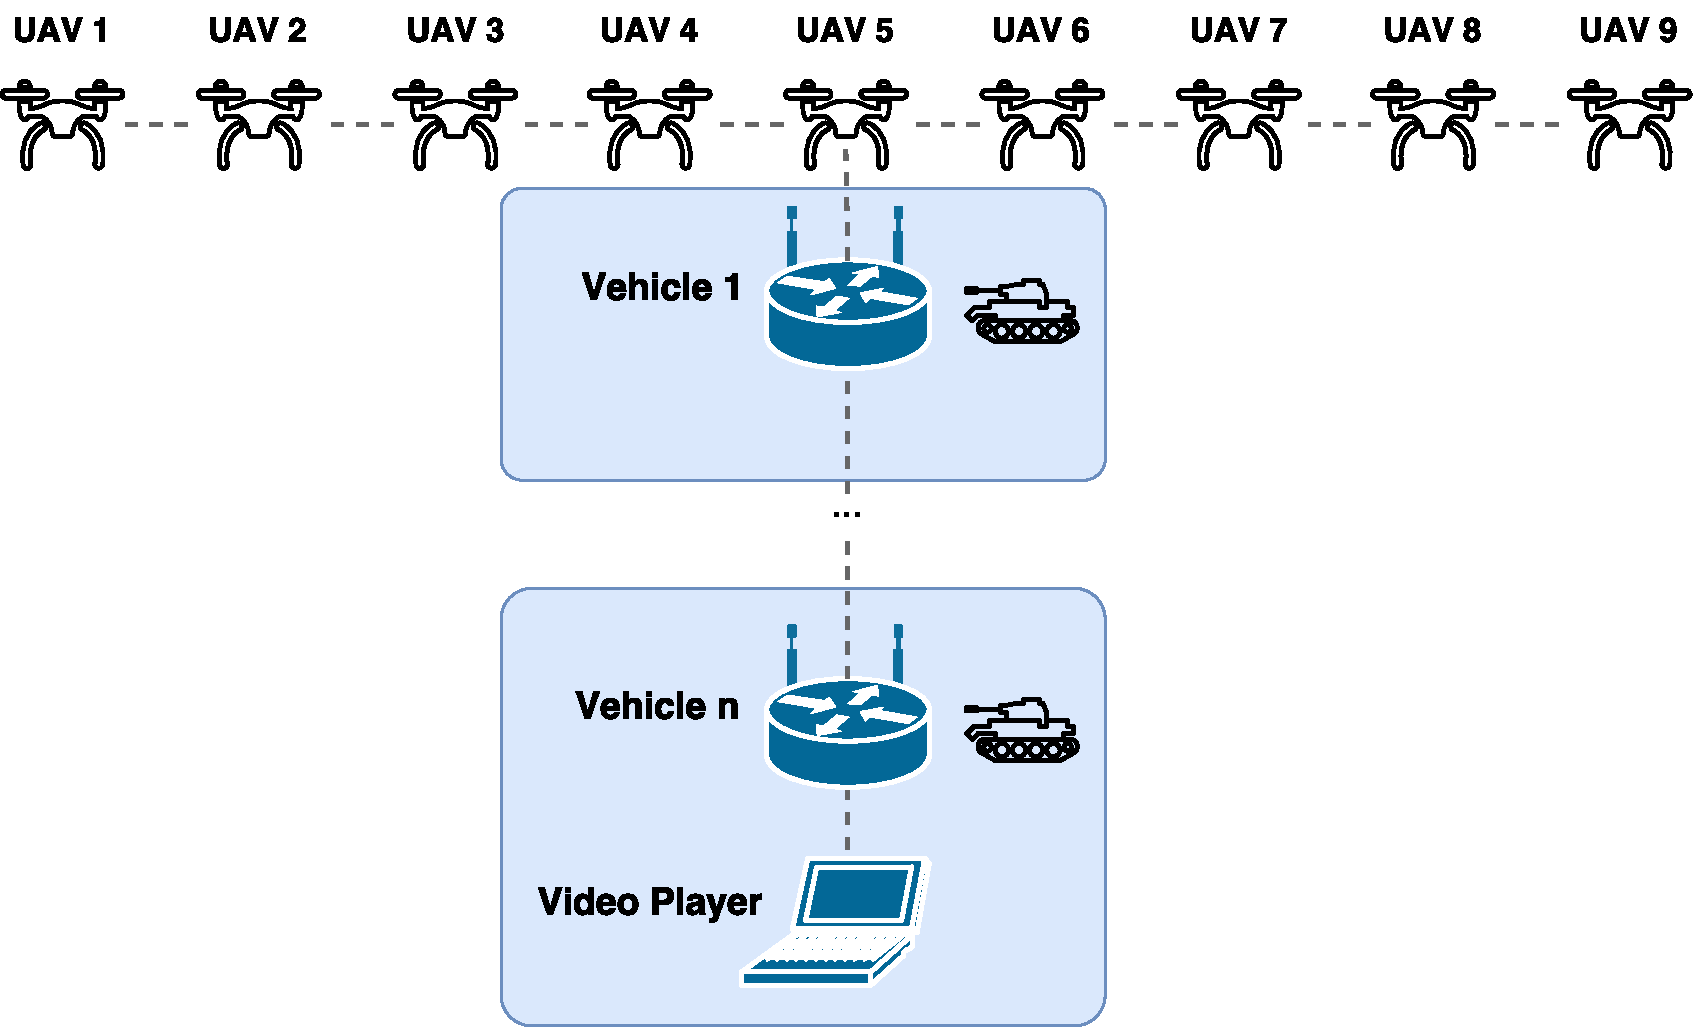
\includegraphics[scale=0.2]{images/forcas_armadas_1.pdf}
        \tiny
        \caption{Dashed and dotted lines represent communication links among Unmanned Aerial Vehicles and Ground Vehicles}
    \end{figure}
\end{frame}

% ----------------------------------------------------------------
\begin{frame}{Links and Problem Characterization}
\begin{itemize}
  \item Links
      \begin{itemize}
          \item Bandwidth (Max. throughput)
          \item Packet loss expected (amount in \%)
        \end{itemize}
  \item Video and Photo format (size, resolution, format)
  \item Mobility of nodes (dynamic behaviour) 
  \item Video client location (The video needs to be accessible from all
  vehicles?)
\end{itemize}
\end{frame}


\section{Implementation}

\subsection{Events Flow Diagram}

% ----------------------------------------------------------------
\begin{frame}{Flow Diagram of Topology Discover}
  \begin{columns}
    \begin{column}{0.5\textwidth}
      \begin{figure}
	    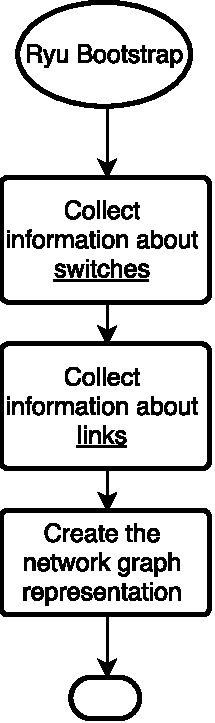
\includegraphics[scale=0.45]{images/algorithm0.pdf}
	    \caption{Topology discovering process}
	  \end{figure}
    \end{column}
    \begin{column}{0.5\textwidth}
      \begin{itemize}
      \item Wait for Ryu topology start-up
      \item Use of LLDP Messages for discovering
      \item Create a network representation using NetworkX
      \end{itemize}
    \end{column}
  \end{columns}
\end{frame}

% ----------------------------------------------------------------
\begin{frame}{Flow Diagram of Packet In}
  \begin{columns}
    \begin{column}{0.5\textwidth}
      \begin{figure}
	  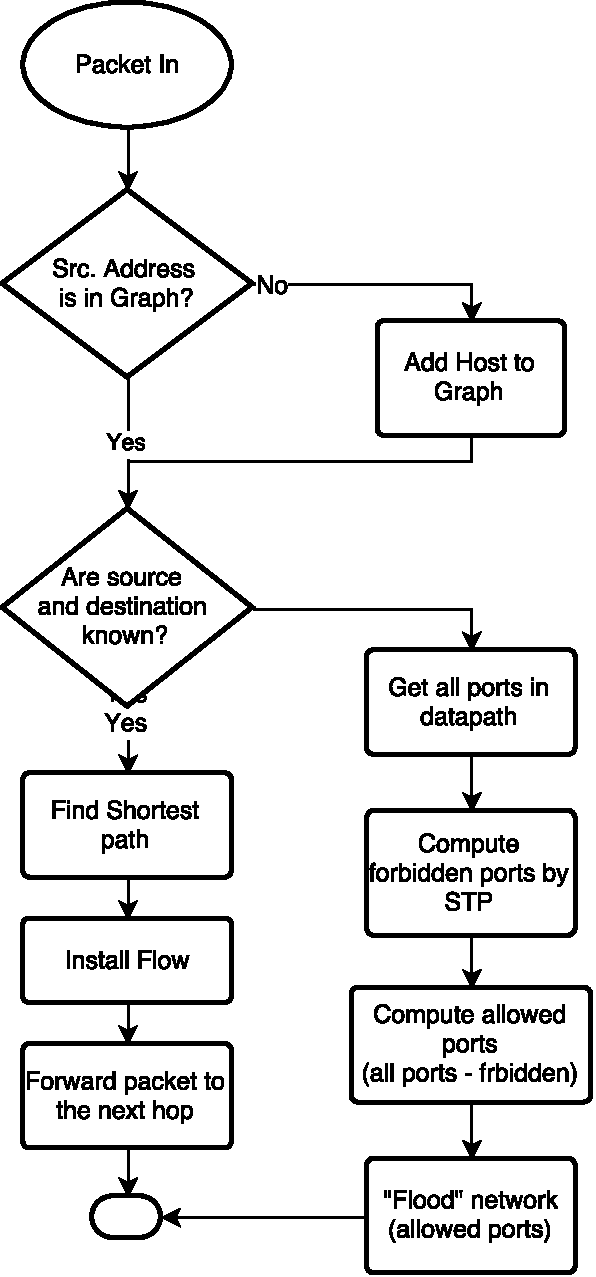
\includegraphics[scale=0.27]{images/algorithm1.pdf}
	  \caption{Overview of Packet In event}
	  \end{figure}
    \end{column}    
    \begin{column}{0.5\textwidth}
      \begin{itemize}
      \item Discover new hosts
      \item Find shortest path (known destination host)
      \item Discover destination using ARP messages
      \item Broadcast of ARP in ``controlled'' network path
      \item Discover of destination on ARP Response
      \end{itemize}
    \end{column}
  \end{columns}
\end{frame}

% ----------------------------------------------------------------
\begin{frame}{Flow Diagram of Port Status Change}
  \begin{columns}
    % Column 1    
    \begin{column}{0.5\linewidth}
      \begin{figure}
	    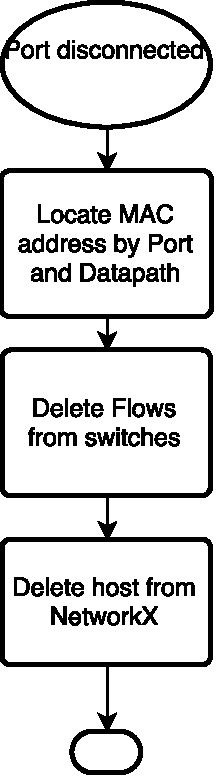
\includegraphics[scale=0.45]{images/algorithm2.pdf}
	    \caption{Topology discovering process}
	  \end{figure}
    \end{column}
    % Column 2  
    \begin{column}{0.5\linewidth}
      \begin{itemize}
      \item OpenFlow sends an ``Port disconnected'' message
      \item Locate hardware address traversing the NetworkX graph
      \item Delete flows from switches in old path
      \item Delete the host disconnected from graph (NetworkX)
      \end{itemize}
    \end{column}    
  \end{columns}
\end{frame}

\subsection{Tools and libraries}
% ----------------------------------------------------------------
\begin{frame}{Tools and Libraries Employed}
\begin{itemize}
  \item ``Mininet'' used to simulate networks, hosts and topology
  \item Controller developed using Ryu Framework (v: 4.3)
  \item OpenFlow (v: 1.3.x) and Open vSwitch(**)
  \item Video playback and metrics using VLC Media Player
  \item NetworkX library for graph manipulation
\end{itemize}
\end{frame}

\section{Results}


\subsection{ARP Broadcast Messages}
% ----------------------------------------------------------------
\begin{frame}{ARP Messages forwarded}
  \begin{figure}
    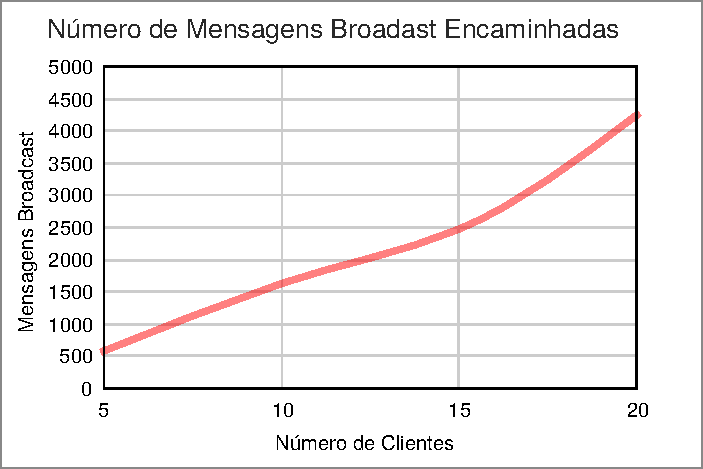
\includegraphics[scale=0.45]{images/graph_bcast.pdf}
    \caption{Amount of forwarded ARP Broadcast*}
  \end{figure}
\end{frame}

\subsection{OpenFlow Messages}

% ----------------------------------------------------------------
\begin{frame}{OpenFlow Rules}
  \begin{figure}
    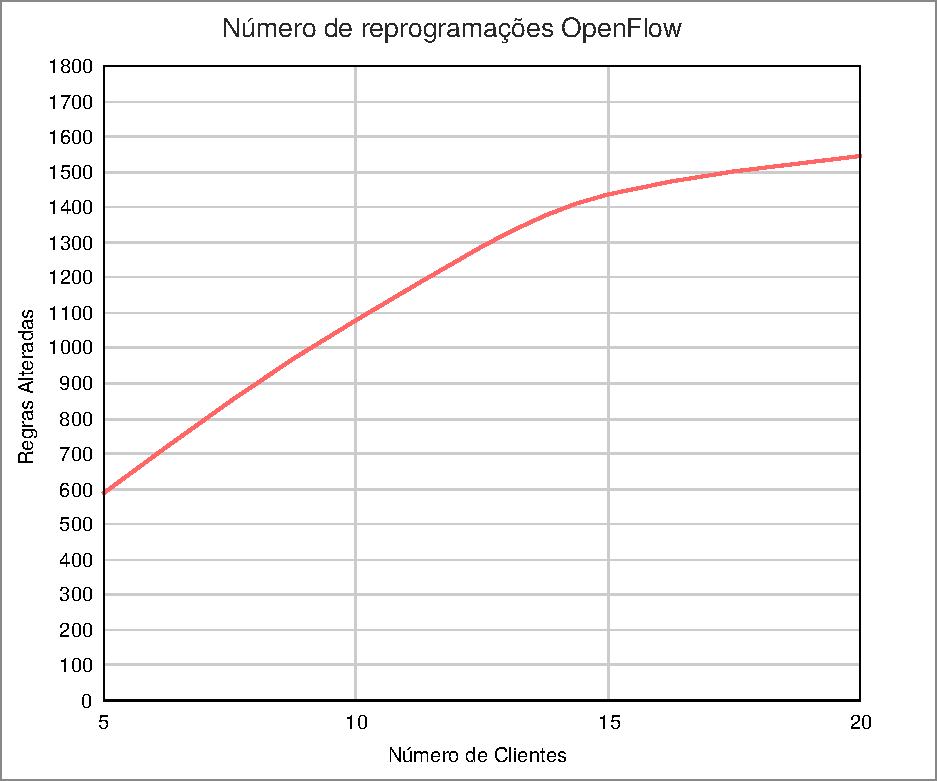
\includegraphics[scale=0.32]{images/graph_of.pdf}
    \caption{OpenFlow reprogramming rules}
  \end{figure}
\end{frame}


\section{Conclusion}

% ----------------------------------------------------------------
\begin{frame}{Conclusion}
\begin{itemize}
  \item Mobility simulation using Mininet offer some challenges
  \item Open vSwitch is not fully compatible with OpenFlow 1.3
  \item Traditional Spanning Tree Protocol (IEEE 802.1D) is not 
        suitable for high mobility scenario
\end{itemize}
\end{frame}

% ----------------------------------------------------------------
\section{References}
\begin{frame}{References}
\begin{thebibliography}{Schroeder, 1991}
\footnotesize
\bibitem{Schroeder1991}
  Bob Lantz, Brandon Heller, and Nick McKeown.
  \newblock Network in a Laptop: Rapid Prototyping for
            Software-Defined Networks.
  \newblock{\em 9th ACM Workshop on Hot Topics in Networks}, Oct. 20-21
  \newblock Monterey, CA.
  
\bibitem{Peak1994}
  Aric A. Hagberg, Daniel A. Schult and Pieter J. Swart.
  \newblock Exploring network structure, dynamics, and function using NetworkX
  \newblock{\em in Proceedings of the 7th Python in Science Conference}, p. 11--15, Aug. 2008.
  \newblock Pasadena, CA
  
\bibitem{Peak1994}
  Nippon Telegraph and Telephone Corporation
  \newblock Ryu SDN Framework
  \newblock https://osrg.github.io/ryu/ 
\end{thebibliography}
\end{frame}

\end{document}




